\section{Results}
\label{sec:results}

% Goal : demonstrate the robustness to 

The goal of this section is to quantify the performance of our \ac{LTR} framework when deployed in the environment described in~\autoref{sec:env}.
We achieve this by evaluating the localization accuracy of the \ac{ICP} algorithm through various metrics.
We also show our camera and \ac{GNSS} measurements to demonstrate navigation approaches using these sensors as primary mean of localization would suffer significant performance loss in a subarctic forest.
Afterwards, we evaluate the path-following performance of our controller and quantify our \ac{UGV}'s energy consumption for each run.
Lastly, we identify failure cases for our system and they were handled in the field.

\subsection{Localization}
\label{sec:res_loc}

\lightlipsum[1]

\subsubsection{Vision-based}
\label{sec:res_vis}

The Dalsa C1920 camera allowed us to analyze the feasibility to use this type of sensor in a subarctic forest. As it was observed by ~\citep{Williams2009} and ~\citep{Paton2017}, the use of cameras for robotic purpose in winter conditions is extremely difficult because of the lack of features on snow terrain. As depicted in~\autoref{fig:cameras_b}, the only features available are the ones from the trees and the surroundings. The path totally recovered by snow is flat and without texture.~\citep{Paton2017} also observed that lighting changes can alter the quality of the image and sunlight reflection on snow can saturate the camera sensor. Their observations related to lighting changes was based on the variation of the sun position during the day, but, in our case, the illumination changes inside the same path. In~\autoref{fig:cameras_a}, there is an example from the TeachA where the quality of the image is sufficient while the robot is in the wood, but can drastically changes if there is an opening in the canopy. In those situations, the camera's sensor is overexposed.

Data were also taken during a snowfall to see the effect on image's quality. As we can observed in~\autoref{fig:cameras_b}, snowflakes are circled in red and are practically invisible in the camera image. Another problem with the use of cameras for vision-based localization comes from the lack of luminosity at night as depicted in~\autoref{fig:cameras_c}. The robot needs to be equipped with its own source of light to travel in the dark compared to lidar which is independent to the lighting conditions.

\begin{figure}[htpb]
	\begin{center}
		\begin{subfigure}[b]{0.32\textwidth}
			\includegraphics[width=\linewidth]{figs/camera/figure_camera_teachA_top.pdf}
		\end{subfigure}%
		~
		\begin{subfigure}[b]{0.32\textwidth}
			\includegraphics[width=\linewidth]{figs/camera/figure_camera_run9_top.pdf}
		\end{subfigure}
		~
		\begin{subfigure}[b]{0.32\textwidth}
			\includegraphics[width=\linewidth]{figs/camera/figure_camera_dark_top.pdf}
		\end{subfigure}%
		\\ \vspace{2mm}
		\begin{subfigure}[b]{0.32\textwidth}
			\includegraphics[width=\linewidth]{figs/camera/figure_camera_teachA_bottom.pdf}
			\caption{TeachA}
			\label{fig:cameras_a}
		\end{subfigure}%
		~
		\begin{subfigure}[b]{0.32\textwidth}
			\includegraphics[width=\linewidth]{figs/camera/figure_camera_run9_bottom.pdf}
			\caption{R8}
			\label{fig:cameras_b}
		\end{subfigure}
		~
		\begin{subfigure}[b]{0.32\textwidth}
			\includegraphics[width=\linewidth]{figs/camera/figure_camera_dark_bottom.pdf}
			\caption{Night}
			\label{fig:cameras_c}
		\end{subfigure}%
	\caption{Pictures taken for three different runs. (a) is an example of the sun's effect on the quality of the images. (b) were taken during a snowfall (most prominent snowflakes are circled in red). Images depicted in (c) were taken at night, hence the lack of luminosity.} 
	\label{fig:cameras_expo}
	\end{center}
\end{figure}

\subsubsection{GNSS}
\label{sec:res_gnss}

As explained in the previous sections, \ac{GNSS} positionning was not used for the teach and repeat because of the lack of precision of the \ac{GNNS} in cluted environnement such as fores trails.

\autoref{fig:gnss_error_path} shows some qualitative examples of positionning error given along the path A and Bd during the run 4 and 5.
On the bottom right side picture, we can clearly see that the \ac{GNSS} positionning is not good in the garage when the run start. 
This is due to the few number of satellite seen by the antennas and the lack of signal received to do the localization accurately.
Others pictures in this figure show some miss-alignement of the path of the robot into the forest trails.
The path computed by the \ac{GNSS} are located into the trees and not on the forest trail.

After this quanlitative analyzis, we also did a quantitative analyzis of the \ac{GNSS} error obtained for each run and according to each path.
The \ac{GNSS} error can be estimated by taking the computing distance between the two antennas and compare it to the one measured by a precise instrument such as a total station \citep{Vaidis2021}.
For each run, we computed this distance for each timestamp of the \ac{GNSS} data and substract it by the theoritical one.
\autoref{fig:gnss_run_error} shows the box plot of the \ac{GNSS} error for each run and with their conresponding path.
We can observe that some paths produced a different spread of the error.
It's the case for the path C, where the precision of the \ac{GNSS} is very high compare to the one of the path B.
Also, for some paths the errors in localization can be higher than the width of the forest trails.
Because of this, the teach and repeat would not have worked properly if our localization was based on \ac{GNSS} positionning.
This quantitative analyzis confirms the observations done with the qualitative analyzis.

By relying only on \autoref{fig:meteo_all}, we are not able to give the reason of the error difference observed for each path and run.
Based on \autoref{fig:gnss_satellite_number}, we can give some answers.
This figure represents some boxplot about the satellite number seen by the \ac{GNSS} antennas during each run for each path.
The number varie between 2 to 21.
The run C has the highest average number of satellite seen during its runs.
This can explain why the precision of the \ac{GNSS} is higher than the other paths.
For the run 4, 2, 6 and 9, we can also link the result of the \ac{GNSS} precision to the number of satellites seen.
In these runs, the number was lower in average than the other runs, which leads to an increase of the uncertainty about the localization as seen in \autoref{fig:gnss_run_error}.
For all the others runs, their results are almost the same with an accuracy around 1 meter and a good precision.



\begin{figure} [htpb]
	\centering
	\includegraphics[height=2.5in]{./figs/GPS/GNSS_numsatvserr.pdf}
	\caption{GNSS satellite number for each run.}
	\label{fig:gnss_satellite_number}
\end{figure}

\begin{SCfigure}
	\centering
	\includegraphics[height=3.0in]{./figs/GPS/GNSS_numsatimg.pdf}
	\caption{GNSS error for each runs.}
	\label{fig:gnss_run_error}
\end{SCfigure}


\subsubsection{ICP}
\label{sec:ICP}

\lightlipsum[1]

\begin{figure} [htpb]
	\centering
	\includegraphics[height=1.6in]{example-image}
	\caption{Figure explaining ICP error for every run (correlated with meteo).}
	\label{fig:icp_error}
\end{figure}



\subsection{Motion and control}
\label{sec:res_motion}

In order to characterize the performance of our path-following controller, we computed the cross track error for each measured position in each repeat run.
Our definition of the cross-track error is the distance between the robot frame $\robotf$'s origin and it's orthogonal projection on the path, as defined in~\citep{Mondoloni2005}.
The results for the cross-track error are displayed in~\autoref{fig:pf_error}.
It can be seen that for all trajectories, the cross-track error mostly remains below \SI{0.1}{m} for most of the runs.
Path curvature can be correlated with an increased cross-track error, with a maximum observed error of \SI{0.8}{m}.
In terms of different runs, it can be observed that cross-track error is stable, despite varying meteorological conditions. 

\begin{figure}[htpb]
	\begin{center}
		\begin{subfigure}[b]{\textwidth}
			\centering
			\includegraphics[height=2.5in]{figs/ref_traj_errors.pdf}
			\caption{Mean cross-track error with respect to the reference trajectories.}
			\label{fig:pf_error_traj}
		\end{subfigure}
		\\
		\begin{subfigure}[b]{\textwidth}
			\centering
			\includegraphics[height=2.0in]{figs/cur_vs_crosstrack.pdf}
			\caption{Cross-track error for all runs.}
			\label{fig:pf_error_runs}
		\end{subfigure}
		\caption{Cross-track error during the deployment.
		The cross-track error was computed for every localization position recorded during each repeat run.
		For each map, the coordinates are defined in the reference map frame $\mapf$, which are the same as shown in~\autoref{fig:ref_ltr}.} 
		\label{fig:pf_error}
	\end{center}
\end{figure}


\begin{figure} [htpb]
	\centering
	\includegraphics[height=2.0in]{example-image}
	\caption{Power consumption / motion efficiency figure.}
	\label{fig:moiton_power}
\end{figure}

\subsection{Failure cases}
\label{sec:fail}
%% Discuss Laverdiere failure and garage failure

\subsubsection{Corridor effect}
\label{sec:forest_canyon}

\lightlipsum[1]

\begin{figure}[h!]
	\begin{center}
		\begin{subfigure}[b]{0.3\textwidth}
			\includegraphics[width=\linewidth]{figs/forest_canyon/run5_perturbations.pdf}
			%\caption{A view from above the \textit{Montmorency} forest, which covers \SI{400}{km^2}.}
			\label{fig:R5_pert}
			\caption{R5}
		\end{subfigure}%
		~
		\begin{subfigure}[b]{0.3\textwidth}
			\includegraphics[width=\linewidth]{figs/forest_canyon/run6_perturbations.pdf}
			%\caption{An example of a snowy path, in which our system performed \ac{LTR}.}
			\label{fig:R6_pert}
			\caption{R6}
		\end{subfigure}%
		~
		\begin{subfigure}[b]{0.3\textwidth}
			\includegraphics[width=\linewidth]{figs/forest_canyon/run2_perturbations.pdf}
			%\caption{An example of a snowy path, in which our system performed \ac{LTR}.}
			\label{fig:R2_pert}
			\caption{R2}
		\end{subfigure}%
		~
		\begin{subfigure}[b]{0.065\textwidth}
			\includegraphics[width=\linewidth]{figs/forest_canyon/colorbar.pdf}
			%\caption{An example of a snowy path, in which our system performed \ac{LTR}.}
			\label{fig:R2_pert}
			\caption{R2}
		\end{subfigure}%
		%% Maybe change with a camera image?
		\caption{Mean residual error after longitudinal perturbation of $^{\lidarf} \readpc$, when matched on $^{\lidarf} \refpc$.
		The perturbations were done from \SI{-6}{m} to \SI{-6}{m}, with increments of \SI{0.5}{m}.
		The maps were built with 500 point clouds for each run that were spread evenly time wise, with the color proportional to the mean perturbation error.
		} 
		\label{fig:forest_canyon}
	\end{center}
\end{figure}

\subsubsection{Run 10 failed initialization}
\label{sec:laverdiere_fail}

\lightlipsum[1]

\begin{figure}[tpbh!]
	\begin{center}
		\begin{subfigure}[b]{0.3\textwidth}
			\includegraphics[width=\linewidth]{figs/run10_init_fail/run_6.pdf}
			%\caption{A view from above the \textit{Montmorency} forest, which covers \SI{400}{km^2}.}
			\label{fig:r6_pcl}
			\caption{R6 (Mean error = \SI{0.0607}{m})}
			\vspace{0.2in}
		\end{subfigure}%
		~
		\begin{subfigure}[b]{0.3\textwidth}
			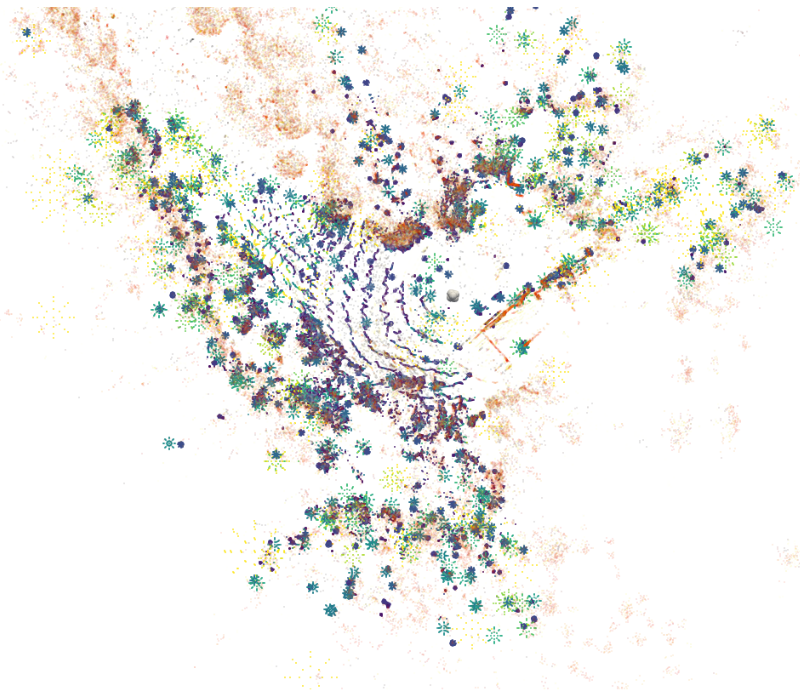
\includegraphics[width=\linewidth]{figs/run10_init_fail/run_10.pdf}
			%\caption{An example of a snowy path, in which our system performed \ac{LTR}.}
			\label{fig:r10_pcl}
			\caption{R10 (Mean error = \SI{0.1072}{m})}
			\vspace{0.2in}
		\end{subfigure}%
		~
		\begin{subfigure}[b]{0.3\textwidth}
			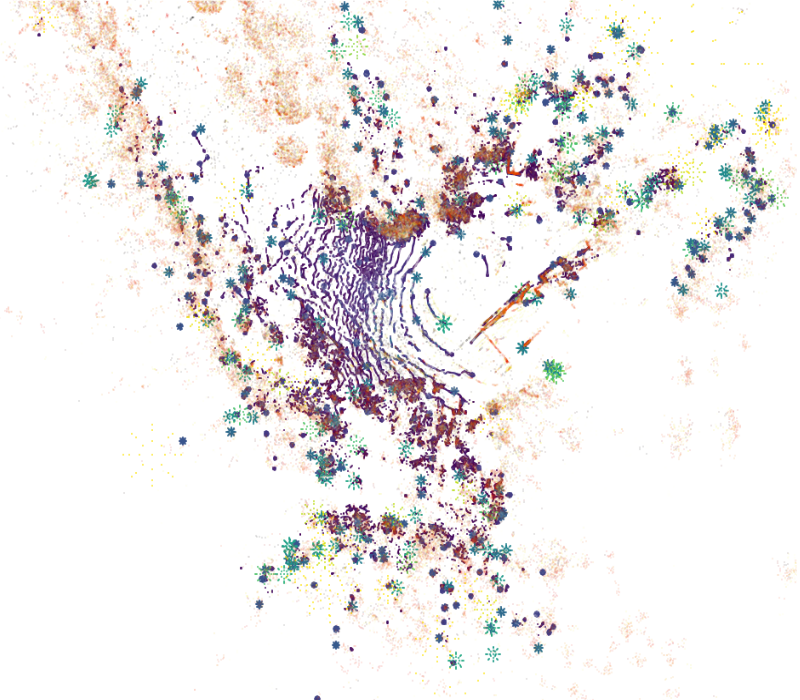
\includegraphics[width=\linewidth]{figs/run10_init_fail/run_15.pdf}
			%\caption{An example of a snowy path, in which our system performed \ac{LTR}.}
			\label{fig:r15_pcl}
			\caption{R15 (Mean error = \SI{0.0698}{m})}
			\vspace{0.2in}
		\end{subfigure}%
		~
		\begin{subfigure}[b]{0.07\textwidth}
			\includegraphics[width=\linewidth]{figs/run10_init_fail/colorbar.pdf}
			%\caption{An example of a snowy path, in which our system performed \ac{LTR}.}
			\label{fig:cbar_run10}
			\vspace{0.2in}
		\end{subfigure}%
		\\
		\begin{subfigure}[b]{0.45\textwidth}
			\includegraphics[width=\linewidth]{figs/run10_init_fail/run10_init.pdf}
			\caption{Camera view of R10 initialization.}
			\label{fig:r10_cam}
		\end{subfigure}%
		~
		\begin{subfigure}[b]{0.45\textwidth}
			\includegraphics[width=\linewidth]{figs/run10_init_fail/run15_init.pdf}
			\caption{Camera view of R15 initialization.}
			\label{fig:r15_cam}
		\end{subfigure}%
		%% Maybe change with a camera image?
		\caption{Initial scans for R6, R10 and R15, with the camera view for R10 and R15 (no camera images were recorded during R6).
		Our \ac{LTR} system was unable to localize within the reference map at the start of R10.
		After multiple attempts, we managed to successfully initialize the run and were able to repeat it completely autonomously.
		Snow accumulation in R10 on the ground creates a significant change in perspective for the lidar, causing a much higher registration error than the other.} 
		\label{fig:icp_failure_r10}
	\end{center}
\end{figure}